% !TeX spellcheck = en_GB

%% =============================================================== %%
%%   5th ECCOMAS International Conference on			           %%
%%	 Inverse Problems Methods  									   %%
%%   22nd - 24th May, 2019, Rzeszow-Kombornia, Poland              %%
%% =============================================================== %%

\documentclass{ShortPaper_Instructions_LaTeX_IPM2019}

% This class will provide automatically the formatting options required
% The class loads automatically the following packages: hyperref, calc,
% indentfirst, url, graphicx, polski, inputenc, qtimes
% In order to obtain a pdf file, the following options are available:
% 1. process file with pdflatex
% 2. process file with latex+dvipdfm
% 3. process file with latex+dvips, and convert to pdf with distiller or other

\usepackage[OT1,OT4]{fontenc}
\usepackage[utf8]{inputenc} % Windows code page (cp1250), for Unicode type use 'utf8' (if necessary)

\title{INSTRUCTIONS FOR PREPARING TWO PAGE ABSTRACTS}

\author{Adam Marsza\l ek$^{1,\ast}$}

\address{$^1$Institute of Computer Science, Computational Intelligence Department,\\
Cracow University of Technology, Warszawska 24, 31-155 Cracow, Poland\\
e-mail: amarszalek@pk.edu.pl}

\begin{document}

\section{INTRODUCTION}
\noindent Two page abstracts (short papers) should outline the main assumptions, models and algorithms formulation, original results, final conclusions and possible applications. In this paper the main relevant references should be quoted, e.g. [1-3]. The above listed information will be taken into account at the reviewing of the abstract.

Authors are invited to submit electronically their abstracts, through the web site of the Symposium, \textbf{before February 15th, 2019}. The Abstract can be submitted directly in its final form. Authors will have the possibility of replacing the file by an updated version after the acceptance notification, but this will not be a requirement.

\section{ABSTRACT PREPARATION}
\noindent The Abstract should be written following the format of the Latex and Word template for submission that can be found in the website: http://ipm.prz.edu.pl/. The file must be converted to Portable Document Format (PDF) before submission through the Conference website. Other formats are not accepted by the Organizers.

The Abstract must contain the full name and full address of author(s). In the case of joint authorships, the name of the author who will actually present the paper at the Conference should be indicated with an asterisk. Papers can only be accepted on the understanding that they will be presented at the Conference.

The Abstract must be written in English within a printing box of 130mm x 205mm, centered in the page. Please do not paginate your abstract. Maximum file size is 4~MB.

\section{EQUATIONS, FIGURES AND TABLES}
\noindent Equations, figures and tables must be centred and numbered sequentially:
\begin{eqnarray}
	\mathbf{K q}=\lambda \mathbf{P}^\ast .
\end{eqnarray}
Figures and tables should also include a small description label (as indicated in Fig.~\ref{fig:fig1} and Table~\ref{tab:tab1}) and should be referred within the text. All mentioned components must appear within the designated margins whereas illustrations will be reproduced in gray scale.
\begin{figure}[t]
\begin{center}
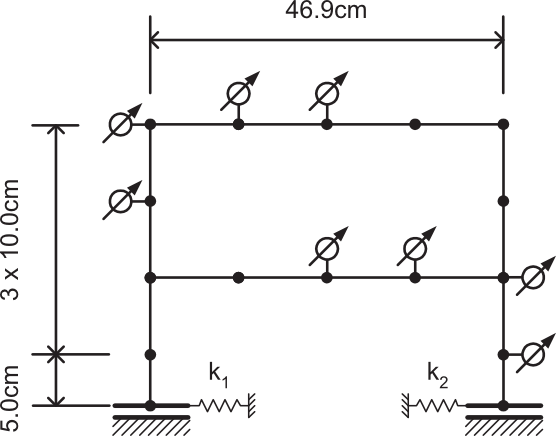
\includegraphics[width=6cm]{frame_model.png}
\caption{Example of a figure.}
\label{fig:fig1}
\end{center}
\end{figure}

\begin{table}[ht]
  \begin{center}
  \caption{Eigenvalues and eigenvectors of covariance matrix \textbf{S}.}
  \label{tab:tab1}
    \begin{tabular}{*{4}{c}}
    \hline
    No. of PC & Eigenvalues & Coeff. 			& Eigenvectors \\
    $j$ 			& $\lambda_j$ & $m_j$ (\%) 	& $\mathbf{q}_j$ \\
    \hline
    1 & 32.029 & 0.9516 (95.1) &	\{ 0.0852,  0.0589,  0.0019,  0.9946 \}	\\
    2 & 1.548 & 0.0460   (4.6) &	\{-0.3472, -0.9339, -0.0072, -0.0850 \}		\\
    3 & 0.081 & 0.0024   (0.2) &	\{ 0.9339, -0.3526,  0.0070, -0.0592 \}		\\
    4	&	0.001	& 0.0000   (0.0) &	\{ 0.0092,  0.0044, -0.9999,  0.0009 \}	\\
    \hline
    \end{tabular}
  \end{center}
\end{table}

\section{FINAL REMARKS}
\noindent Please note that final acceptance of papers for presentation is conditional to receiving the Abstract and the payment of the presenting author's congress registration fee. Only one presentation per delegate is allowed.

\textbf{Important}: Before submitting the contribution you should be registered. Please fill in the registration form using your e-mail address as login and choosing your password. Please type the e-mail carefully since you will not be able to repair it after registration. To modify any other information or add/modify the file of the Abstract you have to log-in. Registration does not oblige contributors to pay the fees before having received the acceptance letter.

For any question, please do not hesitate to contact IPM 2019 Secretariat: ipm@prz.edu.pl.

\begin{thebibliography}{99}

\bibitem{Zienkiewicz} O.C. Zienkiewicz, R.C. Taylor,
\textit{The finite element method, Vol. I, 4th Edition}. McGraw Hill, 1989.

\bibitem{Oden} J.T. Oden, T. Belytschko, I. Babuska, T.J.R. Hughes,
Research directions in computational mechanics.
\textit{Computer Methods in Applied Mechanics and Engineering}, \textbf{192}, 913--922, 2003.

\bibitem{Argyris} J.H. Argyris, M. Papadrakakis, L. Karapitta,
Elastoplastic analysis of shells with the triangular element TRIC.
M. Papadrakakis, A. Samartin, E. Onate eds.
\textit{4th International Colloquium on Computation of Shell and Spatial Structures}, 463--486,
Chania, Crete, Greece, June 4-7, 2000.

\end{thebibliography}

\end{document}
